\section{Geradores ótimos}

\section{Vetorização do diagrama de persistência}
Dado uma sequência de conjuntos de dados $X_i$ e os respectivos diagramas de persistência tem-se uma variação no
seus tamanhos, devido a natureza do algoritmo de homologia persistente. Além de variação entre os tamanhos, cada 
diagrama é um multi-conjunto, sendo mais difícil de analisar-los. Ao utilizar algoritmos de machine learning, 
assume-se entradas com tamanhos fixos no conjunto inteiro de dados. Portanto diagramas de persistências descrevendo
uma sequência de proteínas, por exemplo, precisam ser vetorizados de alguma forma antes de podermos utilizar em
conjunto com outros algoritmos, como redes neurais ou regressão linear. 

Existem várias formas de vetorização de um diagrama de persistência, como \textit{Persistence landscapes}
\cite{bubenik15a} e Imagem de persistência (\textit{Persistence Image}) \cite{Adams2017}. Neste trabalho apresentamos
a imagem de persistência e alguns exemplos.

\subsection{Estabilidade da Imagem de Persistência}
Imagem de persistência é uma vetorização de forma que o respectivo diagrama é representado como 
uma imagem de tamanho fixo $(n,m)$. De forma intuitiva esse método é uma forma de suavização do diagrama 
de persistência, em que uma gaussiana é centrada em cada ponto e depois são somadas com peso. Abaixo descrevemos
formalmente o processo para obter uma imagem de persistência.

Seja $D = \Set{(b_i,d_i)}_{i}$ um diagrama de persistência em alguma dimensão e considere $T(x,y) = (x, y-x)$ 
uma transformação linear em $\mathbb{R}^2$. Seja $T(B)$ o multiconjunto decorrente da transformação linear $T$
aplicada em $B$ onde cada ponto $(x,y) \in B$ corresponde ao ponto $(x,y-x) \in T(B)$. Considere agora uma 
função de probabilidade diferenciável $\phi_u\colon \mathbb{R}^2 \to \mathbb{R}$ com média $u=(u_x, u_y)$. 

Fixe agora uma função peso $f\colon \mathbb{R}^2 \to \mathbb{R}$ de tal forma que ela é zero no eixo horizontal,
contínua e diferenciável por partes. É importante que essas condições sejam satisfeitas, pois elas garante
a estabilidade da imagem de persistência sob a distância $1$-Wasserstein. Dessa forma temos a seguinte definição. 

\begin{defi}
    Para um diagrama de persistência $B$, a correspondente superfície de persistência $\rho_B \colon \mathbb{R}^2
    \to \mathbb{R}$ é a função dada por 
    \begin{equation*}
        \rho_B(z) = \sum_{u \in T(B)} f(u) \phi_u(z). 
    \end{equation*}
\end{defi}

Entretanto, um computador não consegue utilizar uma função para fazer cálculos e estimativas, ela precisa
ser vetorizada (ou discretizada) de alguma forma. Desta forma, vamos discretizar $\rho_B$ em um domínio específico,
que depende de $T(B)$. Em específico, fixamos um grid e o valor de cada pixel é dado pela integral nessa região.

\begin{defi}
    Seja B um diagrama de persistência. A imagem de persistência de B é a coleção de pixeis 
    \begin{equation*}
        I(\rho_B)_p = \iint_p \rho_B dydx.
    \end{equation*}
\end{defi}

Na vetorização do diagrama alguns parâmetros precisam ser estabelecidos. Em \cite{Adams2017} mostra-se que
as imagens são robustas sob a escolha da resolução (tamanho do grid). A outra escolha é a distribuição e dependendo
a variância. Em \cite{Adams2017} a distribuição gaussiana é utilizada com variância dependendo do problema e 
sendo assim o usuário a escolhe. Por último, a escolha da função peso, que pode variar de problema pra problema.
A função abaixo é um exemplo utilizado por \cite{Adams2017}. Observe que para pontos com valores altos de 
persistência tem um valor maior também. Mas com problemas que pontos de baixa ou média persistência são importantes,
a utilização de outros pontos se faz necessária. 

\begin{equation}\label{eq:weightfunct}
    w_b(t) = \left\{
             \begin{array}{@{}ll@{}} 
                 0           & \text{ if } t \leq 0, \\
                 \frac{t}{b} & \text{ if } 0 < t < b, \\
                 1           & \text{ if } t \geq b, 
             \end{array}\right.
\end{equation}
onde $b$ é considerado o valor de maior persistência em $T(B)$.

Em vários conjuntos é normal que apresentem ruídos e algumas variações, assim dando diagramas de persistência
diferentes. Entretanto, há uma medida para avaliar a distância entre eles. 
\begin{defi}
    A distância $p$-Wasserstein definida entre dois diagramas de persistência B e B' é dada por 
    \begin{equation*}
        W_p(B,B') = \inf_{\gamma\colon B \to B'} \left( \sum_{u\in B} \norm{u - \gamma(u)}_{\infty}^{p} 
                    \right)^\frac{1}{p},
    \end{equation*}
    onde $1 \leq p < \infty$ e $\gamma$ é bijeção entre $B$ e $B'$. 
\end{defi}

Seja $h\colon \mathbb{R}^2 \to \mathbb{R}$ uma função diferenciável. Denote 
$\mid \nabla h \mid = \sup_{z\in \mathbb{R}^2} \norm{\nabla h(z)}_2$. Pelo teorema do valor médio, temos que 
\begin{equation}\label{eq:mean_val}
    \mid h(u) - h(v) \mid \leq \mid \nabla h \mid \norm{u-v}_2.
\end{equation}

Seja $u,v\in \mathbb{R}^2$ e considere as duas distribuições diferenciáveis $\phi_u, \phi_v$. Como o supremo e 
a derivada de direção maximal de uma distribuição de probabilidade diferenciável são invariantes por translação,
podemos denotar $\mid \nabla \phi_u \mid$ por $\mid \nabla \phi \mid$ e $\norm{\phi_u}_\infty$ por
$\norm{\phi}_\infty$. E observe ainda devido a invariância pela translação, temos que 
\begin{equation}\label{eq:mean_val_dist}
    \norm{\phi_u - \phi_v}_\infty \leq \mid \nabla \phi \mid \norm{u-v}_2.
\end{equation} 

Vamos enunciar um lema agora que será utilizado nas provas de estabilidade das imagens de superfície e persistência.

\begin{lem}\label{lema:persimg}
    Sejam $u,v\in \mathbb{R}^2$, temos que $\norm{f(u)\phi_u - f(v)\phi_v} \leq 
    \left( \norm{f}_\infty \mid \nabla \phi \mid + \norm{\phi}_\infty \mid \nabla f \mid \right) \norm{u-v}_2.$
\end{lem}
\begin{demonstracao}
Seja $z\in \mathbb{R}^2$ qualquer, então
\begin{align*}
  \begin{split}
    \abs{f(u)\phi_u(z) - f(v)\phi_v(z)} &= \abs{f(u) \left(\phi_u(z) - \phi_v(z)\right) + \left( f(u) - f(v)\right)
    \phi_v(z)} \\
    &\leq \norm{f}_\infty \abs{\phi_u(z) - \phi_v(z)} + \norm{\phi}_\infty \abs{f(u) - f(v)}\\
    &\leq \norm{f}_\infty \abs{\nabla \phi} \norm{u-v}_2 + \norm{\phi}_\infty + \abs{\nabla f} \norm{u-v}_2 
     \quad \text{por \ref{eq:mean_val_dist} e \ref{eq:mean_val}}\\
    &= \left( \norm{f}_\infty \abs{\nabla \phi} + \norm{\phi}_\infty + \abs{\nabla f}\right) \norm{u-v}_2.
  \end{split}
\end{align*}
\end{demonstracao}

\begin{teo}\label{teo:surf_stab}
  A superfície de persistência é estável em relação a distância $1$-Wasserstein. Dados $B,B'$ diagramas de 
  persistência finitos, temos que 
  \begin{equation*}
    \norm{\rho_B - \rho_{B'}}_\infty \leq \sqrt{10} 
    \left( \norm{f}_\infty \abs{\nabla \phi} + \norm{\phi}_\infty + \abs{\nabla f}\right) W_1(B,B')
  \end{equation*}
\end{teo}
\begin{demonstracao}
  Por hipótese, B e B' são finitos, logo existe uma bijeção entre $B$ e $B'$ que atinge o ínfimo da distância 
  de Wasserstein. Portanto
  \begin{align*}
  \begin{array}{lll}
    \norm{\rho_B - \rho_{B'}}_\infty &= 
                \norm{\sum_{u\in T(B)}f(u)\phi_u - \sum_{u\in T(B)}f(\gamma(u))\phi_{\gamma(u)}}_\infty \\
    &\leq \sum_{u\in T(B)} \norm{f(u)\phi_u - f(\gamma(u))\phi_{\gamma(u)}} & \\
    &\leq \left( \norm{f}_\infty \abs{\nabla \phi} + \norm{\phi}_\infty + \abs{\nabla f}\right) 
            \sum_{u\in T(B)} \norm{u-\gamma(u)}_2 &  \text{por \ref{lema:persimg}}\\
    &\leq \sqrt{2} \left( \norm{f}_\infty \abs{\nabla \phi} + \norm{\phi}_\infty + \abs{\nabla f}\right) 
            \sum_{u\in T(B)} \norm{u-\gamma(u)}_\infty & \text{já que } \norm{\cdot}_2 \leq \sqrt{2} 
            \norm{\cdot}_\infty \text{ em } \mathbb{R}^2 \\
    &\leq \sqrt{10} \left( \norm{f}_\infty \abs{\nabla \phi} + \norm{\phi}_\infty + \abs{\nabla f}\right) 
             \sum_{u\in T(B)} \norm{u-\gamma(u)}_\infty & \text{já que } \norm{T(\cdot)}_2 
             \leq \sqrt{5}\norm{\cdot}_\infty\\
    &=\sqrt{10} \left( \norm{f}_\infty \abs{\nabla \phi} + \norm{\phi}_\infty + \abs{\nabla f}\right) W_1(B,B'). &
  \end{array}
  \end{align*}
A última desigualdade é necessária, pois a distância de Wasserstein é definida sobre os pontos do diagrama de 
persistência que são da forma nascimento e morte, não nascimento e persistência. 
\end{demonstracao}

E por fim, temos que as imagens de persistência são estáveis.
\begin{teo}
    A imagem de persistência é estável em relaçaõ a distância $1$-Wasserstein. Se $A$ é o valor máximo dentre 
    todos os pixeis da imagem, então 
    \begin{equation}
        \norm{I(\rho_B) - I(\rho_{B'})}_\infty \leq 
        \sqrt{10} \left( \norm{f}_\infty \abs{\nabla \phi} + \norm{\phi}_\infty + \abs{\nabla f}\right) W_1(B,B').
    \end{equation}
\end{teo}
\begin{demonstracao}
  A demonstração segue do Teorema \ref{teo:surf_stab} e do fato que para um pixel $p$ qualquer 
  \begin{equation*}
    \abs{I(\rho_B)_p - I(\rho_{B'})_p} \leq A(p) \norm{\rho_B - \rho_{B'}}_\infty,
  \end{equation*}
  em que $A(p)$ representa a área do píxel $p$. 
\end{demonstracao}

\subsection{Exemplos de Imagens de Persistência}
Considere $X$ um conjunto de pontos extraídos de um círculo com ruído, como pode ser visto na 
\autoref{fig:noisycircle}.
\begin{figure}[!htbp]
    \centering
    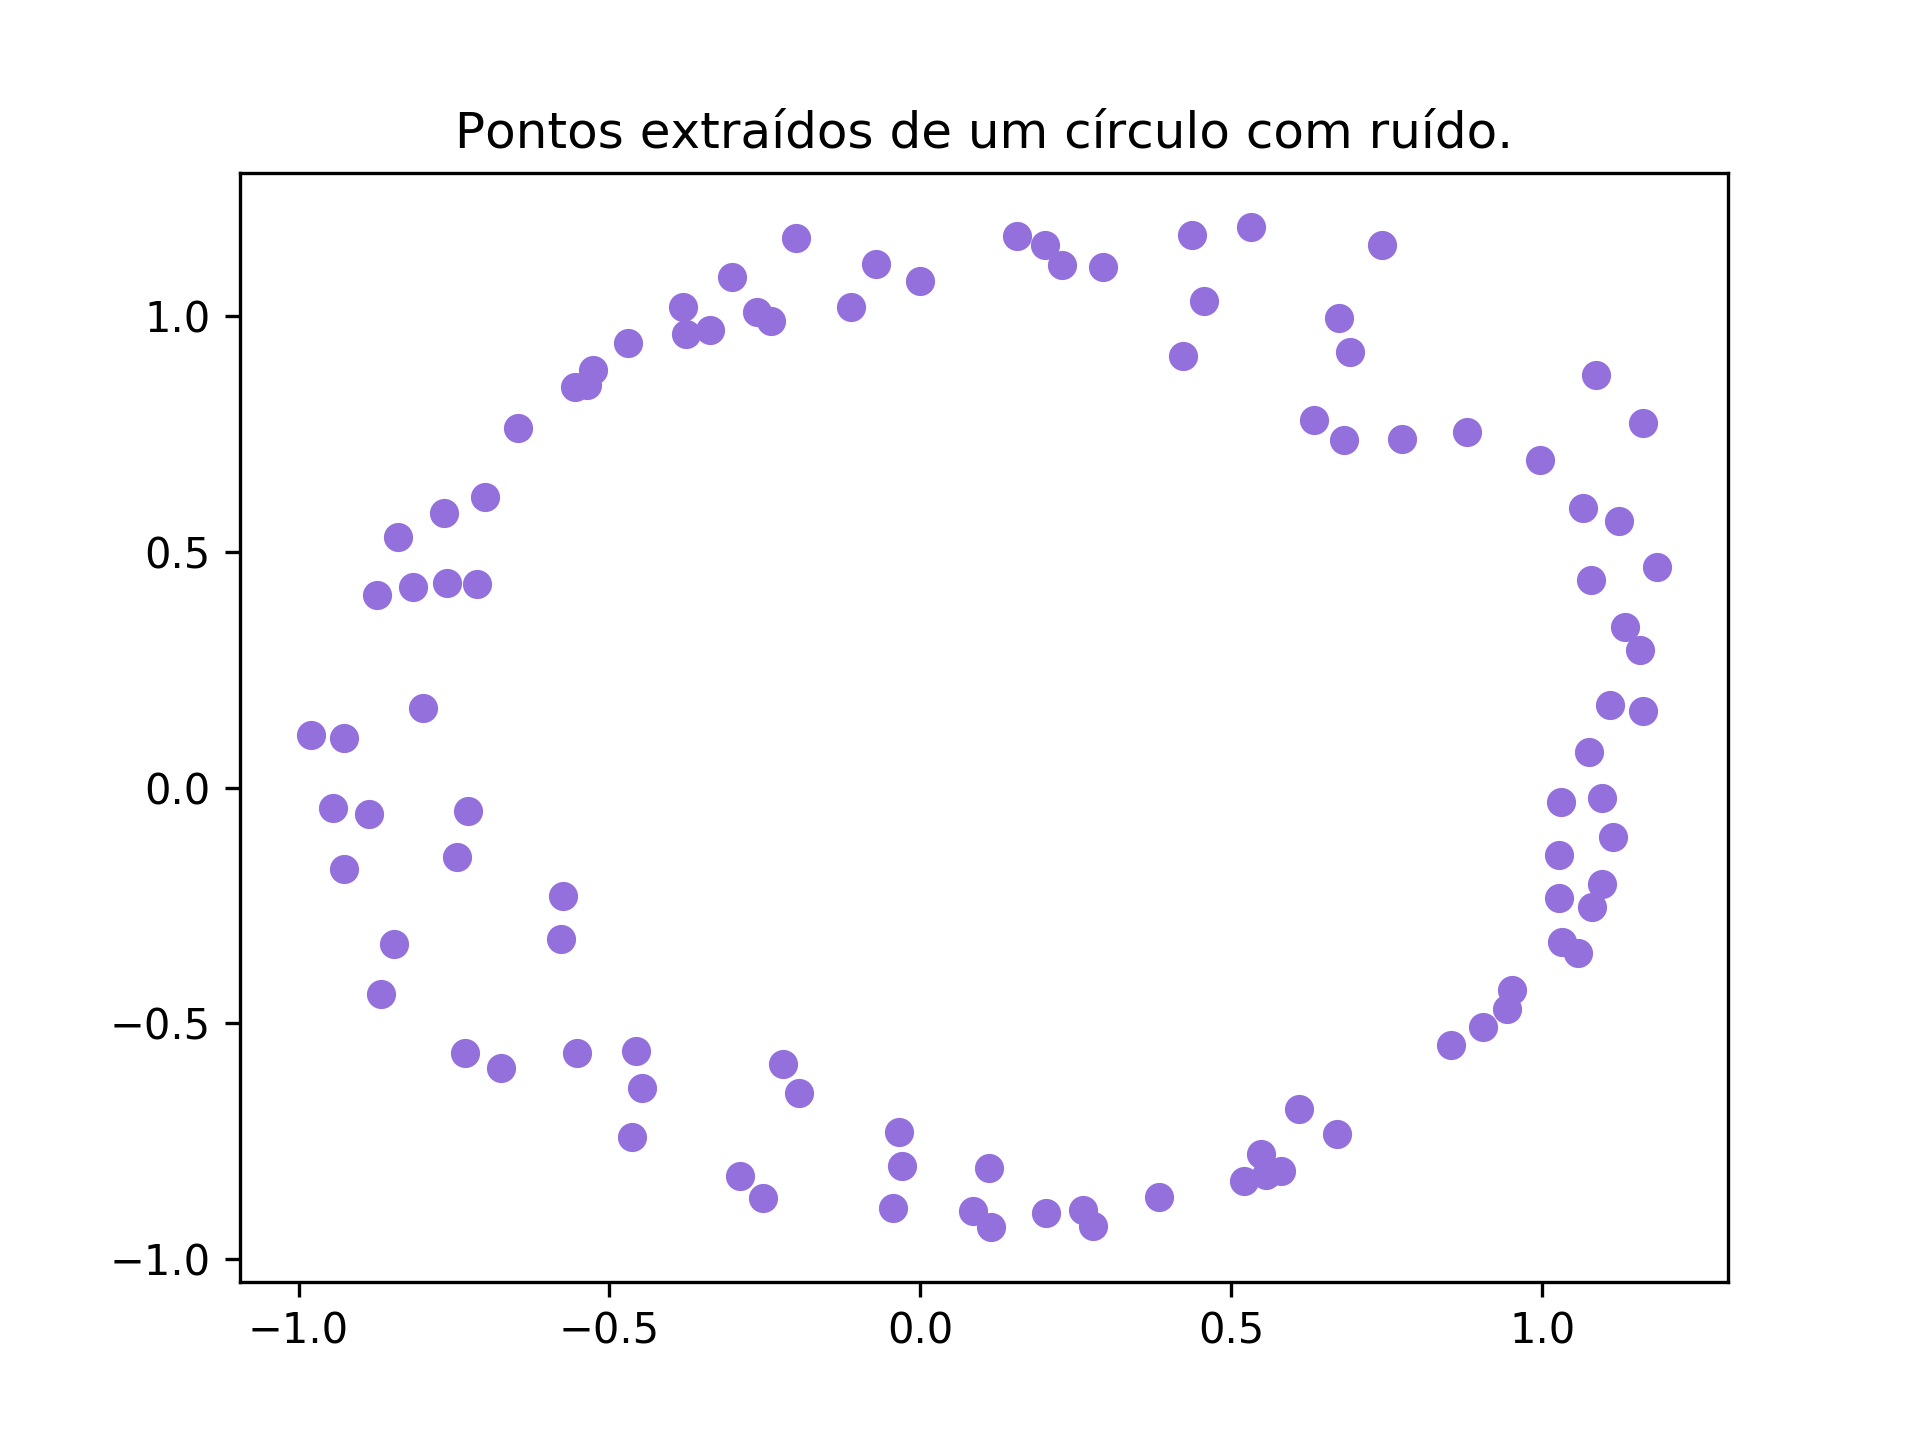
\includegraphics[width=0.7\textwidth]{images/noisy_circle.png}
    \caption{Pontos extraídos de um círculo com ruídos.}
    \fautor
    \label{fig:noisycircle}
\end{figure}
Na \autoref{fig:persdcircle} tem-se os diagramas de persistência do círculo de dimensão $0$ e $1$, assim mostrando
as componentes conexas e buracos. Note que existem dois pontos longe da diagonal, um representando a 
componente conexa e o outro o buraco do círculo.  
\begin{figure}[!htbp]
    \centering
    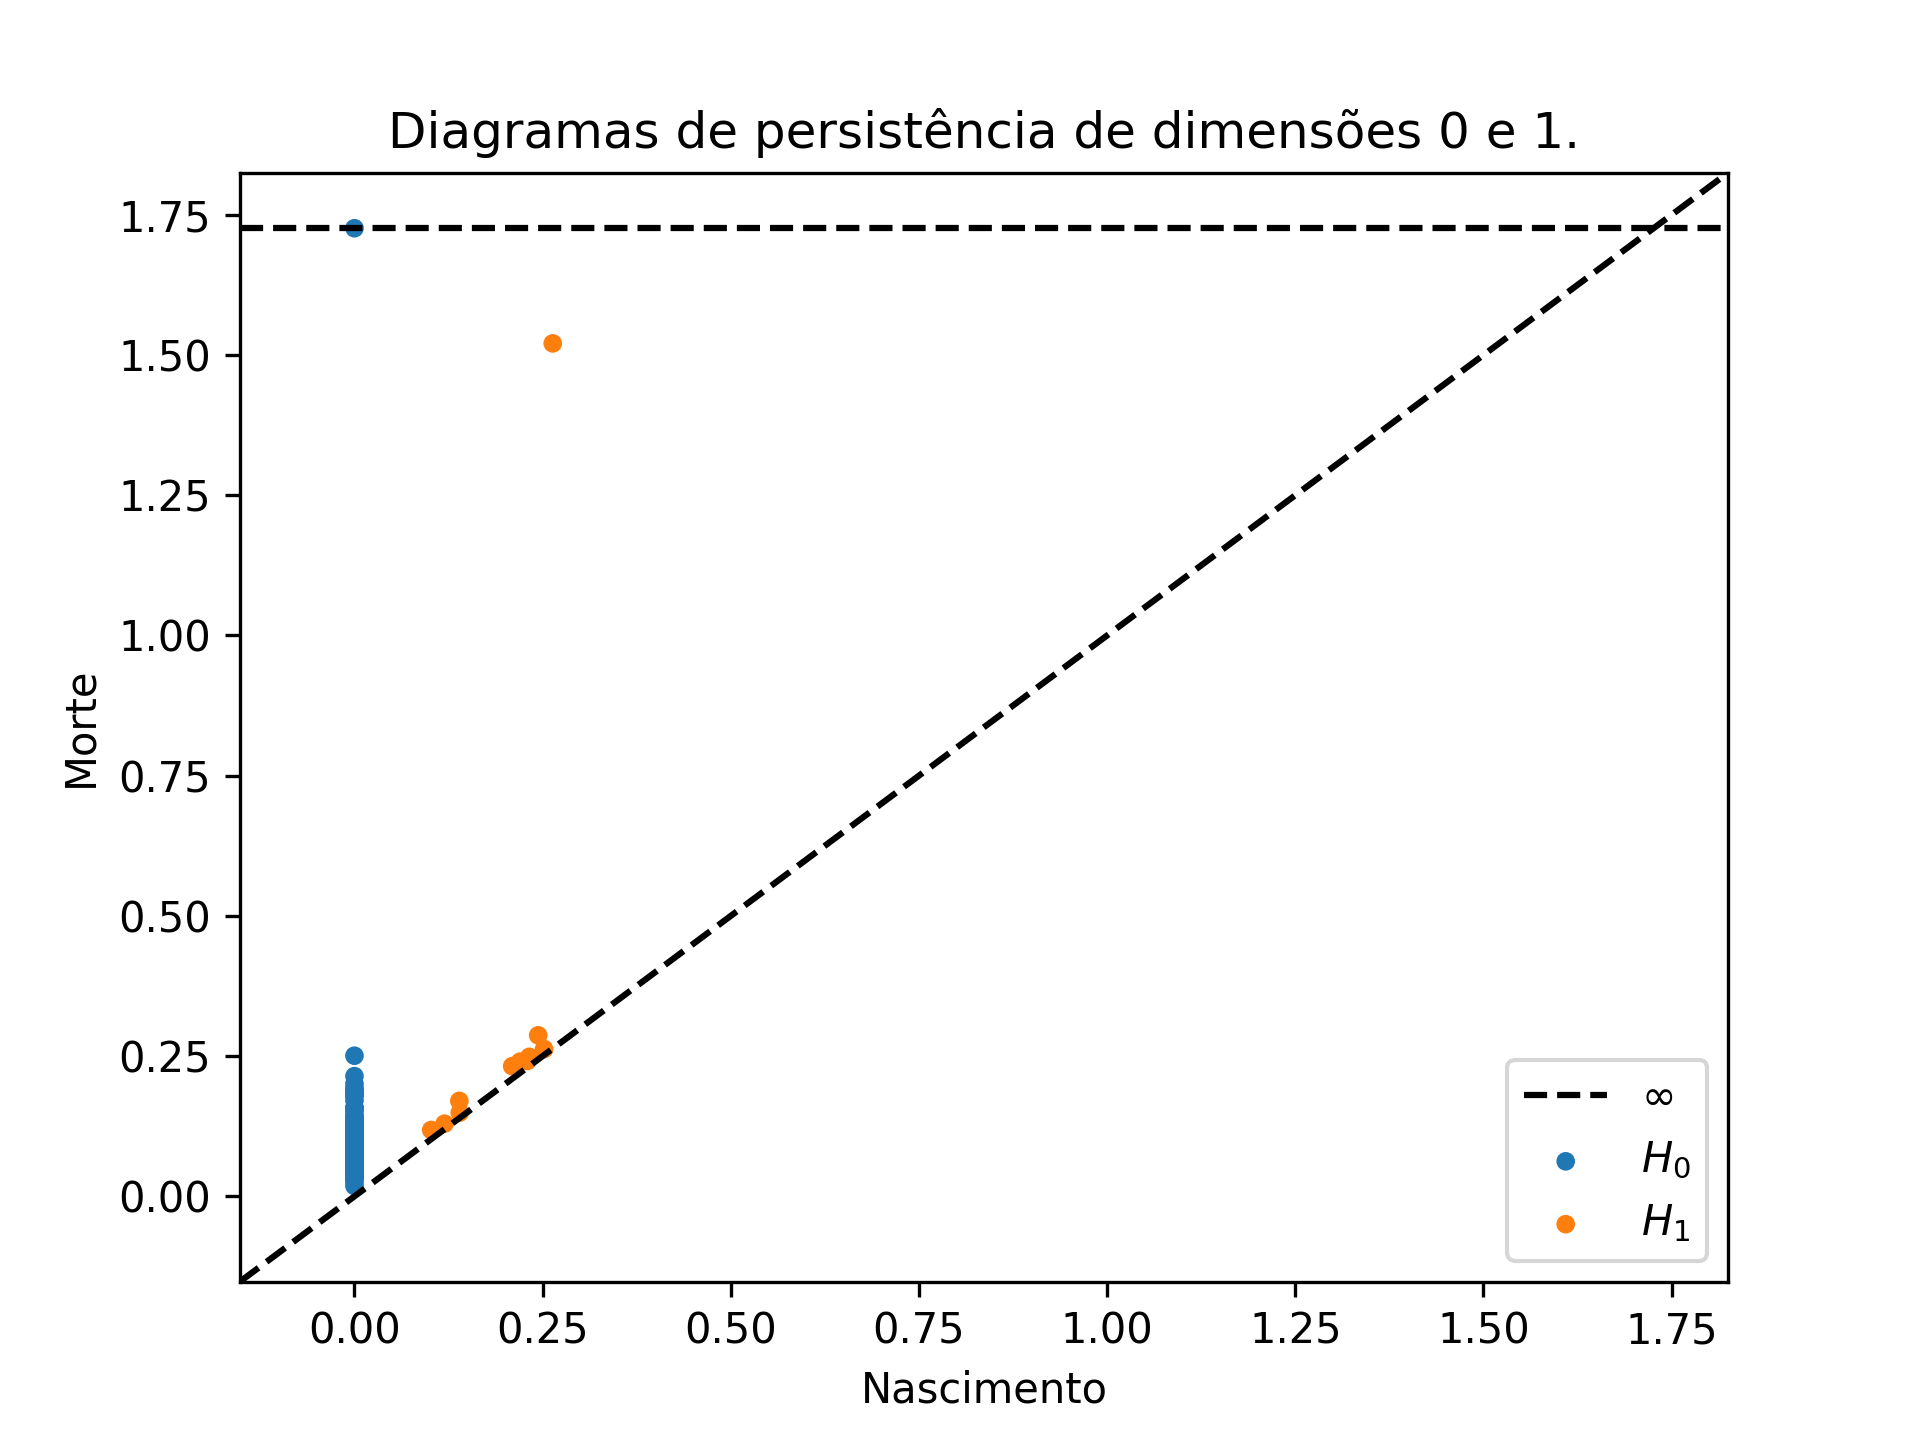
\includegraphics[width=0.7\textwidth]{images/persdcircle.png}
    \caption{Diagrams de persistência do círculo $X$. Em laranja o diagrama de persistência de dimensão $1$,  
            em azul o de dimensão $0$. A filtração de Vietoris-Rips foi usada para calcular o complexo simplicial.}
    \fautor
    \label{fig:persdcircle}
\end{figure}
Vamos agora análisar as imagens de persistência para cada uma das images. Escolhemos a distribuição gaussiana
dada por 
\begin{equation*}
    g_u(x,y) = \frac{1}{2\pi\sigma^2}e^{-((x-u_x)^2 + (y-u_y)^2)/2\sigma^2}.
\end{equation*}
A \autoref{eq:weightfunct} é utilizada como função peso. Para calcular as imagens de persistência 
definimos três variâncias: $0.001, 0.1, 1.0$, e dois tamanhos de imagem: 
$10\times10$ e $50\times50$. O resultado pode ser visto na \autoref{fig:persimgcircle}.
\begin{figure}[!htbp]
    \centering
    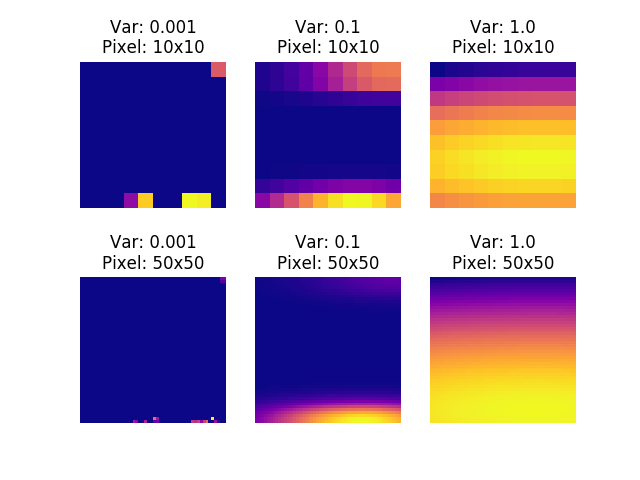
\includegraphics[width=0.9\textwidth]{images/comparacao_pis.png}
    \caption{6 imagens de persistência do diagrama de dimensão $1$ da \autoref{fig:persdcircle}.} 
    \fautor
    \label{fig:persimgcircle}
\end{figure}

Observe a diferença entre os tamanhos escolhidos para as imagens. Com um tamanho maior, a informação fica mais fina,
porém a imagem fica esparsa. Além disso, com uma variância mais baixa os pontos ficam mais concentrados, enquanto
para valores mais altos há uma troca contínua entre as regiões dos pontos com maior frequência.

Todo o código para gerar o círculo com ruído, calcular os diagramas e imagens se encontram no 
\textit{Jupyter Notebook} no repositório da dissertação: \url{https://github.com/chronchi/dissertacao} na pasta
\textit{jupyter\_notebook}.

\section{Mapper}
